\documentclass[
	a4paper, % Paper size, use either a4paper or letterpaper
	10pt, % Default font size, can also use 11pt or 12pt, although this is not recommended
	unnumberedsections, % Comment to enable section numbering
	twoside, % Two side traditional mode where headers and footers change between odd and even pages, comment this option to make them fixed
]{LTJournalArticle}

\usepackage{lettrine}
\usepackage{subcaption}
\usepackage{graphicx}
\usepackage{float}
\usepackage{tikz}
\usetikzlibrary{positioning}

\addbibresource{references.bib} % BibLaTeX bibliography file

\runninghead{Automatic Summarization System} % A shortened article title to appear in the running head, leave this command empty for no running head

\footertext{} % Text to appear in the footer, leave this command empty for no footer text

\setcounter{page}{1} % The page number of the first page, set this to a higher number if the article is to be part of an issue or larger work

%----------------------------------------------------------------------------------------
%	TITLE SECTION
%----------------------------------------------------------------------------------------

\title{Automatic Summarization System} % Article title, use manual lines breaks (\\) to beautify the layout

% Authors are listed in a comma-separated list with superscript numbers indicating affiliations
% \thanks{} is used for any text that should be placed in a footnote on the first page, such as the corresponding author's email, journal acceptance dates, a copyright/license notice, keywords, etc
\author{%
	Christian Faccio\textsuperscript{1} \thanks{\href{mailto:christianfaccio@outlook.it}{christianfaccio@outlook.it}}, 
    Elena Lorite\textsuperscript{1} \thanks{\href{mailto:elenalorite@gmail.com}{elenalorite@gmail.com}},
    Rebeca Piñol Galera\textsuperscript{1} \thanks{\href{mailto:rpg80@alu.ua.es}{rpg80@alu.ua.es}} and 
	Paula Frías Arroyo\textsuperscript{1} \thanks{\href{mailto:pfa13@alu.ua.es}{pfa13@alu.ua.es}}
}

% Affiliations are output in the \date{} command
\date{\footnotesize\textsuperscript{\textbf{1}}University of Alicante}

% Full-width abstract
\renewcommand{\maketitlehookd}{%
	\begin{abstract}
		\noindent In this project we developed an automatic summarization system, which is able to effectively summarize the information present on a set of documents. The process is divided in two steps: information retrieval, done using a non-neural approach with RegEX and a neural approach with transformers, and generation, completed with an encoder-decoder model. We finally analyzed the effectiveness of both approaches, showing that modern state-of-the-art transformers are able to capture more information than standard information retrieval methods, but at the cost of efficiency and possible problems like hallucinations.
	\end{abstract}
}

%----------------------------------------------------------------------------------------

\begin{document}

\maketitle % Output the title section

%----------------------------------------------------------------------------------------
%	ARTICLE CONTENTS
%----------------------------------------------------------------------------------------

\section{Introduction}
\lettrine[findent=2pt]{\textbf{S}}{}ummarizing the text contained in a document is a difficult task even for people. It necessitates the individuation of the most important topics, then the selection of the most important part of them and finally the generation of a smaller text starting from that. 
\textbf{Automatic Summarization Systems} are employed to help in this task: they should be able to summarize the text of the documents autonomously or with limited and small human help like in this case. 
It is a task which divides in two parts: the first is the individuation and extraction of the most important information, while the second is the generation of new text starting from that. 
In our case, the information to be extracted is defined beforehand by us, so the first architecture just needs to find the most relevant parts of the text with respect to that. 
The developed code and relative data can be found in our \href{https://github.com/christianfaccio/automatic_summarization_system.git}{GitHub repository}.

\section{Data}

The documents used in this project are scholarships for students published in the Boletín Oficial del Estado (BOE) and can be found in the \href{https://github.com/christianfaccio/automatic_summarization_system/tree/main/docs}{\texttt{docs/}} folder. They are 5 documents in total and are mostly similar with respect to the format. 

The information extracted is detailed and specific:
\begin{itemize}
	\item academic year;
	\item total budget;
	\item income thresholds;
	\item eligible programs;
	\item scholarship components;
	\item application period;
	\item academic requirements.
\end{itemize}
We believe that this data can represent most of the useful information contained in the documents and a special consideration must be done regarding the type of data extracted, since it is not just common text but comprises ranges, dates, prices and structured information. Given this variety of data types, the information retrieval part had to be specifically tailored for this task, as we will describe in the next section. 
Finally, the extracted information has been written on a JSON file in a structured manner, which can be found in the \href{https://github.com/christianfaccio/automatic_summarization_system/tree/main/output}{\texttt{output/}} folder.


\section{Architecture}

We divided the whole architecture in two components: the \textit{information retrieval (IR)} part and the \textit{generation} part.

The whole architecture and the interaction between components is shown in Figure~\ref{fig:architecture} 


\begin{figure}[h]
	\centering
	\includegraphics[width=0.45\textwidth]{assets/ass.png}
	\caption{General architecture and interaction of components of the developed system.}
	\label{fig:architecture}
	
\end{figure}

\subsection{Information Retrieval}

This was the part in which we spent most time on. Without correct and reliable data, the summarization cannot be done, so this is probably the most important part of the system. There are different methods to be used here, but the most common are the use of \textit{regular expressions}, which are not flexible at all but can extract information with special format like dates, the use of \textit{similarity search} between a query and the chunks of the text, which is more flexible but contains hidden difficulties like the choice of the chunking method, and finally the use of a \textit{transformer} model, which is the state of the art and is flexible, even if costly and complex. 

Even if usually a transformer architecture is the best choice, it may not be for every situation. In fact, the best trade-off between performance and efficiency depends on the caractheristics of the problem at hand. In this case, chunking the text and then use similarity search between a query and them was not the best approach. We, in fact, tried to use a semantic chunker to split parts of the text which are coherent with respect to a speech topic, saved them in a vector store and ran similarity search with the topics of interest. The results were good, the data extracted were coherent with the query, but the main problem was that this way was impossible to extract detailed and structured information as we needed to. This necessity comes from the fact that the documents at hand contain information regarding scholarships, so a summary of them should include detailed information which are helpful for a possible candidate, and that include dates, ranges and mostly numbers. 
Thus, at first glance, a better approach in this specific case is the use of regular expressions. 

We would like to emphasize that this method was possible just because the documents are similar in writing and format, thus the lack of flexibility of the method. But, given that we needed structured and specially formatted information, this was a good approach. The results are shown in the \texttt{info.json} file and are pretty good indeed, even if in some cases we were not able to extract all the data. Unfortunately, with small text variations this method stops working correctly. Figure~\ref{fig:ir_dia} shows a diagram of the RegEx-based information retrieval system.

\begin{figure}[h]
\centering
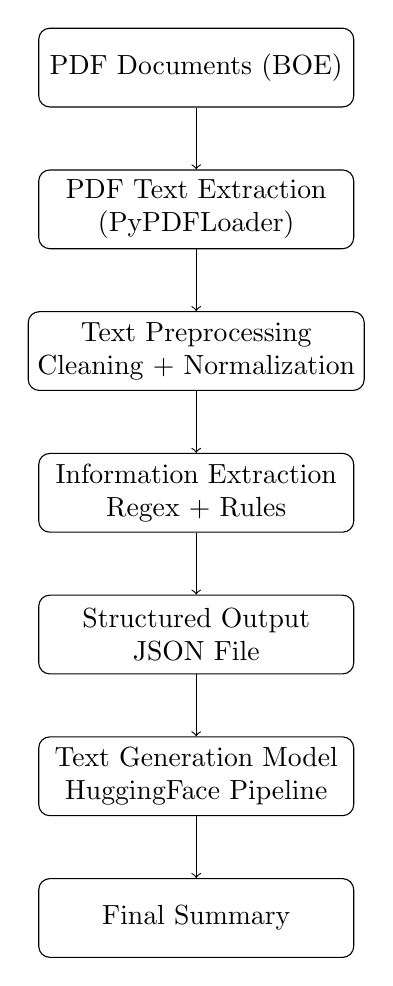
\begin{tikzpicture}[
node distance=1.8cm,
box/.style={rectangle, draw, rounded corners, align=center, minimum width=4cm, minimum height=1cm}
]

\node[box] (pdf) {PDF Documents (BOE)};
\node[box, below of=pdf] (extract) {PDF Text Extraction \\ (PyPDFLoader)};
\node[box, below of=extract] (clean) {Text Preprocessing \\ Cleaning + Normalization};
\node[box, below of=clean] (ir) {Information Extraction \\ Regex + Rules};
\node[box, below of=ir] (json) {Structured Output \\ JSON File};
\node[box, below of=json] (gen) {Text Generation Model \\ HuggingFace Pipeline};
\node[box, below of=gen] (out) {Final Summary};

\draw[->] (pdf) -- (extract);
\draw[->] (extract) -- (clean);
\draw[->] (clean) -- (ir);
\draw[->] (ir) -- (json);
\draw[->] (json) -- (gen);
\draw[->] (gen) -- (out);

\end{tikzpicture}
\caption{System Architecture}
\label{fig:ir_dia}
\end{figure}

We also implemented an alternative approach with a transformer, to see and compare the performance with the former method. With this approach we wanted to evaluate whether a transformer-based model could reduce the amount of the manual logic while improving flexibility and robustness. Unlike the previous method, which relied a lot on rules, regular expressions and specific heuristics, the LLM-based system leaves most of the semantic interpretation to the model itself. First the raw text from the PDF files is extracted and then it is segmented by articles with the use of regular expressions. After, each relevant section is provided to the LLM with a specific prompt for each section. The extracted data from all documents are then combined into a structured file: \texttt{info\_mistral.json}. This approach provided several advantages like higher flexibility and better semantic understanding. However, this approach also has certain downsides: hallucination risk, higher computational cost and output variability. 

To evaluate the impact of model size on performance, we experimented with several open-source LLMs ranging from 3B to 70B parameters (3B, 8B, 14B, 24B, 30B and 70B). As expected, larger models generally produced more accurate and consistent structured outputs, with the 70B model (Llama 3.3) achieving the best performance. However, when considering cost per token, inference latency and overall efficiency, the 24B parameter model (Mistral Small 3.2) offered the best balance between performance and computational cost. Smaller models were capable of completing the task, but their outputs showed a degradation in structural consistency and precision. Based on these experiments, models around 24-30B parameters appear to be the best ones for this type of structured extraction task. 
All inferences for the experimentation were performed through a remote API (OpenRouter), rather than running the models locally. This inference choice simplified experimentation across multiple model sizes. 

Even though medium-sized models seem to be the best for this kind of task, for the final version of the project we have implemented the use of a smaller \textbf{local} model of 3B parameters (Qwen2.5) through the Transformers library as the default option. There is still the option to use the model of 24B parameters through the API by using the \texttt{--use-cloud} argument and passing an API key. Overall the LLM based approach proved to be more adaptable, if needed, and easier to extend to new formats, at the cost of increased computational complexity and potential reliability issues. A diagram representing this LLM-based system can be seen in Figure~\ref{fig:nir_dia}.

\begin{figure}[h]
	\centering
	\includegraphics[width=0.45\textwidth]{assets/nir_diagram.png}
	\caption{Transformers-based information retrieval system.}
	\label{fig:nir_dia}
	
\end{figure}


\subsection{Generation}
We built our summary generation pipeline using open weight instruction tuned language models accessed through Hugging Face Transformers and executed locally. In order to ensure that all group members could run the system on their own hardware, we limited the selected models to approximately 1.7B–3.5B parameters, requiring at most around 6GB of VRAM. The models used in the final version are Phi-3.5-mini-instruct, SmolLM2-1.7B-Instruct, and Qwen2.5-3B-Instruct. These models were chosen because they provide a good balance between computational efficiency and instruction following performance, while remaining lightweight enough for local execution.

Phi-3.5-mini-instruct is a compact but highly optimized instruction-tuned model designed for strong reasoning and controlled text generation. Qwen2.5-3B-Instruct is a more recent instruction aligned model known for stable multilingual and structured generation capabilities. SmolLM2-1.7B-Instruct represents an even smaller architecture, included to evaluate how very lightweight models perform under the same prompting strategy. By comparing these three models, we analyze how differences in parameter scale and architecture influence summary quality.

The summaries were generated from structured JSON data. Each JSON entry was transformed into a designed prompt that explicitly instructed the model to act as an academic writer, produce a structured summary of 200–250 words, and avoid inventing information. The generation process used controlled parameters, including a moderate temperature (0.4), nucleus sampling (top-p 0.9), and a repetition penalty to reduce redundancy. These settings aim to balance determinism and linguistic naturalness and limit variability across runs.

In addition to summary generation, the pipeline incorporates a factual consistency analysis step. A multilingual Natural Language Inference model based on \texttt{mDeBERTa-v3} is used to compute a score between the original structured data (treated as the premise) and the generated summary (treated as the hypothesis). This hallucination score serves as an observational metric to estimate the alignment between the JSON file and the generated summary. We expect Phi-3.5 and Qwen2.5-3B to produce the most coherent and factually consistent summaries due to their stronger instruction tuning, while SmolLM2-1.7B may show more variability given its smaller parameter size.

\section{Evaluation}
The evaluation part of the system asseses three aspects: factual consistency of extracted information, the accuracy of the structured data extraction and the semantic quality of generated summaries. These evaluations will provide an assesment of the system performance across the pipeline.

\subsection{Factual Consistenct Evaluation and Hallucination Detection}
During the neural information retrieval part (transformer-based system), for each extraction task such as the general information, eligible programs, income threshold... hallucination scores are computed This provides factual consistenct metrics per section, so we can identify the sections where the model may have generated hallucinated content. 

To compute hallucination scores, we adopt a section-wise validation strategy. For each extracted field, the model output is aligned with the original source segment from which the information should have been derived. A similarity comparison is then performed between the generated value and the corresponding text span in the document. If no semantically equivalent fragment can be identified in the source, the output is flagged as potentially hallucinated. This method allows us to quantify hallucination likelihood independently for each attribute, rather than evaluating the extraction as a whole. Such fine-grained evaluation is particularly useful because different sections exhibit different linguistic characteristics. For example, numerical sections tend to produce fewer hallucinations than descriptive sections, where models may paraphrase or generalize information. By analyzing hallucination scores per attribute, we obtain a diagnostic view of the neural extraction component and can identify which information categories require stricter prompting or additional validation rules.

\subsection{Structured Data Extraction Evaluation}
Structured extraction accuracy is evaluated by comparing LLM-based extraction (NIR) against regex-based extraction patterns (IR). The IR component is used as ground truth for structured information extraction. This comparative approach allows a quantification of how well the neural extraction methods capture structured information relative to manual patterns.

To ensure fairness, both extraction methods operate over the same cleaned textual input obtained after PDF preprocessing. For each document and each field, the outputs of the neural extractor are compared against those obtained from the rule-based system. A match is counted when the semantic content is equivalent, even if formatting differs. For example, date ranges expressed with different separators or whitespace are considered correct matches. The final accuracy score is computed as the ratio of correctly extracted fields over the total number of expected fields. This evaluation framework allows us not only to measure global accuracy but also to analyze performance per attribute type. In this way, we can identify systematic weaknesses, such as difficulties in extracting multi-clause eligibility requirements or categorizing textual descriptions into predefined labels. This comparison highlights the complementary strengths of both approaches: deterministic reliability from rule-based extraction and semantic flexibility from neural methods.

\subsection{Summary Evaluation}
We evaluate the generated summaries against the original source documents using \texttt{BERTScore}, which is a learned metric based on contextual embbedings from pre-trained models. The evaluation uses \texttt{XLM-RoBERTa-base}, which is a crosslingual variant of the RoBERTa model. This crosslingual model allows meaningful comparison between the Spanish documents and the generated summaries.

The evaluation procedure we followed operates like this: for each language model, all generated summaries across academic years are collected, then the corresponding source texts are extracted from the original PDFs and then BERTScore is computed independently for each summary and source pair. Finally the aggregated performance of each model is computed. This way we have a comparison across models and across documents. The resulting scores are within the range [0, 1]. The closer to 1, the stronger the semantic alignment between summary and source text. Through this metric we can provide a quantitative assesment of how well each model captured the semantic content of the source documents in the summaries.

Together, these evaluation procedures provide a comprehensive assessment of the system across all stages of the pipeline. The hallucination analysis measures factual reliability, the structured extraction comparison quantifies information accuracy, and the BERTScore evaluation assesses semantic fidelity of the generated summaries. By combining these complementary perspectives, we obtain a multidimensional understanding of system performance rather than relying on a single metric.

\subsection{Results and Analysis}
The structured extraction component achieved an overall performance score of 0.713 across all evaluated fields and documents, representing moderate success in capturing scholarship data. However, performance varied across field types. Fields with well defined formatting, like academic year and application period, achieved perfect scores (1.0). The total budget field achieved 0.667, indicating that numeric extraction was generally successful, though one document was skipped due to missing regex ground truth. More linguistically complex fields showed lower performance. The eligible programs field achieved only 0.332, the lowest score. These results show that structured fields containing quantitative data are extracted better than fields requiring categorical assignment.

The three models used for summarization showed consistent performance. Phi-3.5-mini achieved an average BERTScore F1 of 0.793 (range 0.787–0.800), Qwen2.5-3B attained 0.805 (range 0.793–0.813), and SmolLM2-1.7B achieved 0.803 (range 0.786–0.818). These results indicate strong semantic conservation of source document content in the summaries.

Per document analysis reveals small variation, as BERTScore F1 ranged from 0.786 to 0.818 across years and models. The small variation likely reflects the heterogeinity between documents and structure. The consistent ~0.80 performance across years suggests that the summarization pipeline generalizes robustly across different scholarship documents.

These findings suggest that model size was not the dominant factor influencing summary quality, as smaller architectures performed comparably to larger ones. This indicates that the pipeline design and prompt structure likely contributed more to performance stability than raw model capacity. Overall, the results support the robustness of the proposed architecture as a scalable approach for structured document summarization tasks.

\section{Conclusions}
In this work, we presented a hybrid automatic summarization system for structured scholarship documents, combining rule-based information retrieval with transformer-based neural extraction, followed by structured summary generation. The evaluation demonstrates that deterministic methods reliably extract well-formatted fields, while neural methods improve flexibility and capture semantic nuances in more complex sections. 

Factual consistency metrics and hallucination detection reveal that the pipeline maintains high reliability, particularly when using medium-sized models (3B–24B parameters), which offer an optimal balance between performance, efficiency, and computational cost. Smaller models, when properly prompted, also generate coherent and semantically faithful summaries, highlighting the importance of pipeline design and prompt engineering over raw model size.

Overall, the system successfully produces accurate structured data and high-quality summaries across heterogeneous documents, demonstrating its robustness, adaptability, and potential for scalable deployment in structured document summarization tasks.

%----------------------------------------------------------------------------------------
%	 REFERENCES
%----------------------------------------------------------------------------------------

%\nocite{}
\printbibliography % Output the bibliography

%----------------------------------------------------------------------------------------

\end{document}
